% Figure: memory-domain-based ordering (fence) vs completion (quiet).
% Referenced in main_spec.tex as fig:fence-quiet.
% Regenerate PDF/PNG with:  make -C figures
\documentclass[border=3pt]{standalone}
% Shared preamble for the standalone figure sources in this directory.
% Fonts mirror ../utils/packages.tex so the generated figures match the
% specification's typography. tikz pulls in xcolor automatically.
\usepackage[T1]{fontenc}
\usepackage{mathptmx}
\usepackage[scaled=.90]{helvet}
\usepackage{courier}
\usepackage{tikz}
\usetikzlibrary{positioning,arrows.meta,fit,backgrounds,calc}

\begin{document}
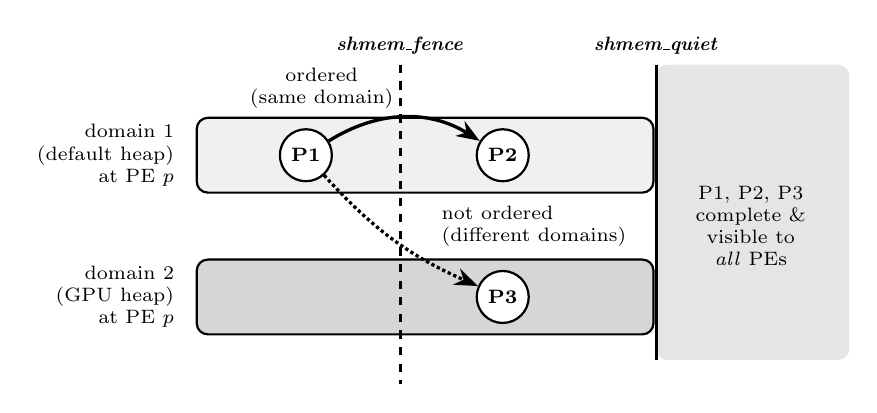
\begin{tikzpicture}[
  font=\footnotesize\sffamily, >=Stealth,
  lane/.style={draw, thick, rounded corners, minimum height=0.95cm},
  opdot/.style={circle, draw, thick, fill=white, minimum size=0.66cm, inner sep=0pt,
                font=\scriptsize\bfseries},
]
  \node[lane, fill=black!6,  minimum width=5.8cm, anchor=west] (d1) at (3.2,0) {};
  \node[lane, fill=black!16, minimum width=5.8cm, anchor=west] (d2) at (3.2,-1.8) {};
  \node[anchor=east, align=right, font=\scriptsize] at (3.05,0)    {domain 1\\(default heap)\\at PE $p$};
  \node[anchor=east, align=right, font=\scriptsize] at (3.05,-1.8) {domain 2\\(GPU heap)\\at PE $p$};

  \node[opdot] (p1) at (4.6,0)    {P1};
  \node[opdot] (p2) at (7.1,0)    {P2};
  \node[opdot] (p3) at (7.1,-1.8) {P3};

  % fence
  \draw[dashed, very thick, black] (5.8,1.15) -- (5.8,-2.9);
  \node[font=\scriptsize\bfseries, anchor=south] at (5.8,1.16) {\textit{shmem\_fence}};

  % ordered: same domain, same PE
  \draw[->, very thick] (p1) to[bend left=32] (p2);
  \node[font=\scriptsize, align=center] at (4.8,0.85) {ordered\\(same domain)};

  % not ordered across domains
  \draw[->, densely dotted, very thick] (p1) to[bend right=12] (p3);
  \node[font=\scriptsize, align=left, anchor=west] at (6.2,-0.9) {not ordered\\(different domains)};

  % quiet
  \begin{scope}[on background layer]
    \fill[black!10, rounded corners] (9.05,1.15) rectangle (11.5,-2.6);
  \end{scope}
  \draw[very thick, black] (9.05,1.15) -- (9.05,-2.6);
  \node[font=\scriptsize\bfseries, anchor=south] at (9.05,1.16) {\textit{shmem\_quiet}};
  \node[align=center, font=\scriptsize] at (10.25,-0.9)
        {P1, P2, P3\\ complete \&\\ visible to\\ \emph{all} PEs};
\end{tikzpicture}
\end{document}
